
% Arxiv styling
% Based on https://github.com/kourgeorge/arxiv-style
\documentclass{article}
\usepackage{arxiv}

\usepackage[utf8]{inputenc} % allow utf-8 input
\usepackage[T1]{fontenc}    % use 8-bit T1 fonts
\usepackage{hyperref}       % hyperlinks
\usepackage{url}            % simple URL typesetting
\usepackage{booktabs}       % professional-quality tables
\usepackage{amsfonts}       % blackboard math symbols
\usepackage{nicefrac}       % compact symbols for 1/2, etc.
\usepackage{microtype}      % microtypography
\usepackage{floatrow}
%\usepackage{natbib}
\usepackage{doi}
\usepackage{graphicx}
\usepackage{subcaption}

% Document
\begin{document}

%% Custom commands
% Inline reference to a hyperparameter.
% Often contains underscores, which must be detokinized
\newcommand{\hyperparam}[1]{\texttt{\detokenize{#1}}}

%% Title
\title{(preliminary title) Model compression for Random Forests using leaf clustering}

%% Author info
\author{
    Jon Nordby \\
	Soundsensing AS \\
	\texttt{jon@soundsensing.no} \\	
}

% Remove the date
\date{}

\maketitle
\renewcommand{\abstractname}{\vspace{-\baselineskip}} % erase the space between authors and abstract

%% Abstract
\begin{abstract}	\noindent
The Random Forest algorithm has been very successful, and continue to be a powerful choice on low-power microcontrollers with small amounts of memory and compute.
Current size-optimized implementations of Random Forest tend to use hard majority voting, where each decision tree returns the most probable class, instead of the class proportions (probabilities).
We show that the hard majority voting rule can lead to a considerable drop in predictive performance on some datasets.
To find a better tradeoff between predictive performance and model size, we propose to use quantization and K-means clustering to adaptively select a small set of class proportions to store for the decision trees.
We evaluate the proposed method on 60 classification datasets from the OpenML CC18 benchmark suite.
Find that only a few class probabilities need to be stored to retain good performance,
with small increase in model size over hard majority voting.
When combined with 16-bit integer quantization of the input features, the method reached average model compression of XX, when staying within XXX percentage point performance drop.
The method is implemented in the open-source TinyML library emlearn, and demonstrated running on microcontrollers for Human Activity recognition tasks.

% Keywords. Maximum 5
\noindent \textbf{Keywords}: Random Forest, TinyML, model compression, tree-based ensemble

\end{abstract}


\section{Introduction}

Big picture motivation.
TinyML use-cases.
TinyML setting. On device inference. Low power. Wireless sensing.

\noindent

\newpage
\section{Background}

\cite{random_forest_breiman2001}

Success cases for Random Forest in TinyML.
Human Activity Recognition. \cite{elsts_are_2021}
Animal behavior. \cite{tatler_high_2018} \cite{kleanthous_feature_2020} \cite{tran_iot-based_2022}

% REGRESSION, not classification Battery monitoring. \cite{mawonou_state--health_2021}

TODO: illustration of tree structure
TODO: illustration of the storage, of decision nodes and leaves
Structure of a random forest.
Decision nodes, leaf nodes.
Voting rules. argmax / Hard majority.
Probability average. Soft.

Fully grown versus partially grown trees.
Fully grown, all leaves with end up with class proportions.
However when there are restrictions. Such as \hyperparam{max_depth}, \hyperparam{min_samples_leaf}, \hyperparam{min_samples_split} etc.
In resource constrained environments, this is the more realistic case.


Class probabilities. 32 bit floating point.
$leaf_size: n_leaves * n_classes * 4 bytes$

Ensemble voting rule:
\begin{verbatim}
probabilities[n_trees, n_classes]
for tree in forest:
   tree_probabilities = predict_tree(tree)
   probabilities[tree] = tree_probabilities
proba = mean(probabilities, axis=1)
\end{verbatim}

As implemented in scikit-learn \cite{scikit-learn} RandomForestClassifier.

Hard majority. argmax. With leaf-deduplication.
Using 1 byte for the class indices, allows up to 255 classes.

$leaf_size = n_classes * 1 * 1 byte$

Voting rule:
\begin{verbatim}
votes[n_classes] = {0,...}
for tree in forest:
   class_index = predict_tree(tree)
   votes[class_index] += 1
out = argmax(votes)
proba = votes / n_classes
\end{verbatim}

As implemented in emlearn 0.9.0 (2019) \cite{emlearn}.

Proposed. Use soft voting rule. Reduce $n_leaves$ using clustering and reduce bitdepth using quantization.

\subsection{Related work}

Optimization techniques for decision trees and decision tree ensembles such as Random Forest has been studied extensively over the last decades, including in a low-power, low-compute setting.

Integer quantization of features.
FPGA/hardware related.
SIMD tree evaluation.

Optimization for microcontrollers \cite{tabanelli_optimizing_2022}
Feature selection. \cite{uddin_guided_2015}, \cite{elsts_energy-efficient_2020}
Early stopping. \cite{daghero_low-overhead_2022} \cite{daghero_adaptive_2021}
Parallelization.
Cache-awareness.

Software tools for deploying RF to TinyML. Open-source


\section{Methods}
What we cover: Feature quantization. Leaf quantization. Leaf clustering.

OpenML CC18 datasets. \cite{oml-benchmarking-suites}
To avoid needing data imputation, the datasets with missing values were ignored.
TODO: list exact identifiers for that which was eliminated

Train a general model. Using scikit-learn. \cite{scikit-learn}
Using 10 trees ({n_estimators}). And {min_samples_leaf=0.01}.
NOTE: clustering will probably save more in percent, the more leaves are used.
Increases both with the number of trees, and the effective depth
- but total model sizes in excess of 100 kB is less relevant for the typical usecase

TODO: consider other values for {min_samples_leaf} ?
Either multiple, or tune on datasets.
It will affect leaf growth.

Metric. AUC ROC one-versus-all.

Numerical variables are scaled using RobustScaler.
Categorical variables are encoded using OrdinalEncoder.

Apply compression strategy to trained model. Re-running predictions on test set.

Cross validation using stratified k-fold.

? Demonstrator of performance on one or few TinyML tasks/datasets.
HAR: PAMAP. UCI DSADS. OPPORTUNITY ? F1 scores. 
Comparisons with other frameworks. Leaf cluster (emlearn), m2cgen, micromlgen
Hardware architectures. ARM Cortex M0+ (no FPU). ESP32 (FPU). Alt: Cortex M4F
TODO: visualization. Panel over HW,dataset of scatterplots with model size and inference time
Need to implement feature computation also.

\footnote{The code for reproducing the experiments can be found at https://github.com/jonnor/leaf-quantization}

\newpage
\section{Results}

0. Baseline for comparison.
TODO: show a plot of the baseline performance?

1. Performance with 16bit and 8 bit feature quantization, vs floating point.
Without any changes to the leaves.
Practically no degradation in performance.
TODO: add some supporting references to 16 bits being enough. Both in general, and specific to decision trees / random forest

\begin{figure}[h!]
\begin{center}
  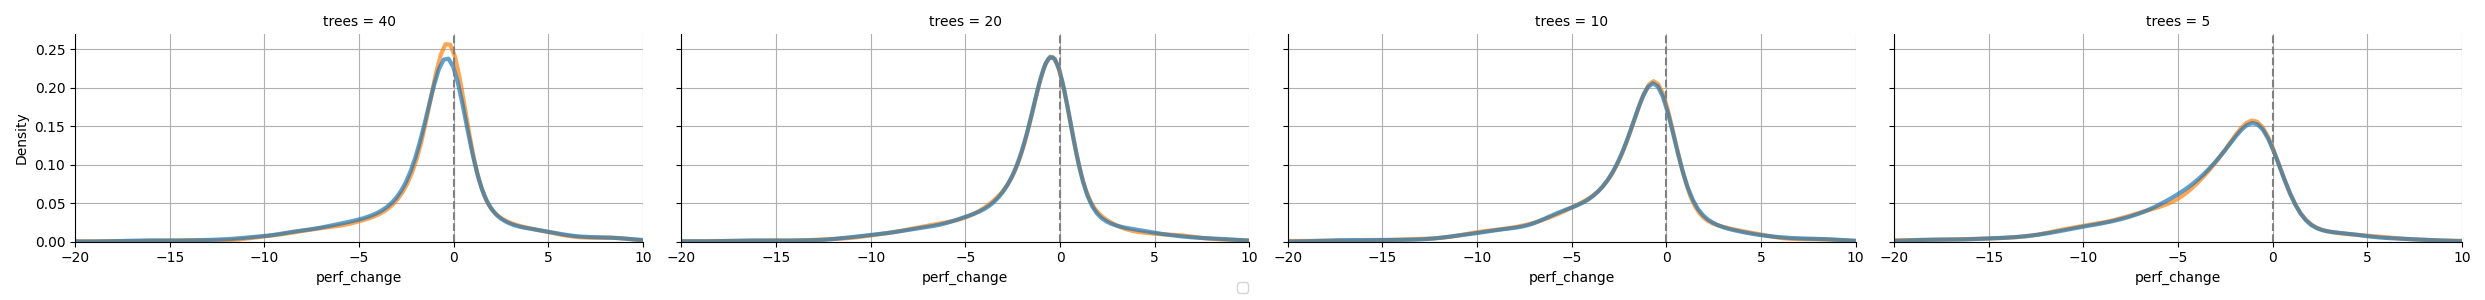
\includegraphics[width=0.98\linewidth]{reports/figures/int16-vs-float.png}
  \end{center}
  \caption{ Performance of different feature representations, relative to the strong baseline model. Computed across all datasets and hyperparameters. 16-bit integer quantized features shows practically identical performance to full precision floating point. }
  \label{fig:int16_vs_float}
\end{figure}

\begin{figure}[h!]
\begin{center}
  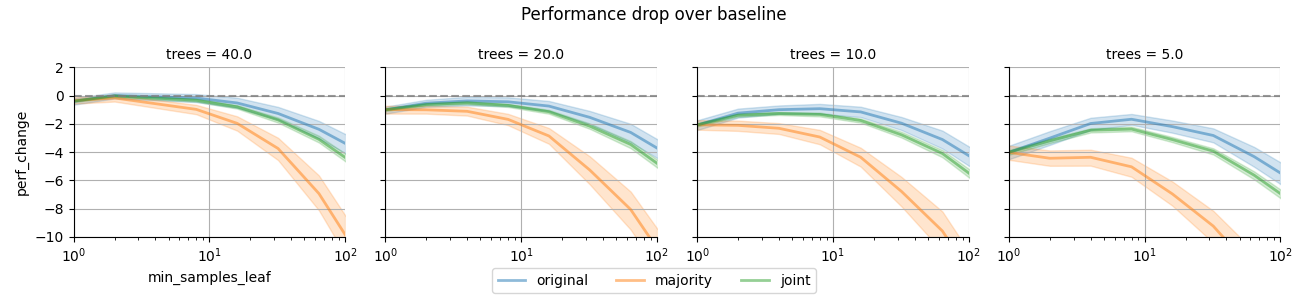
\includegraphics[width=0.98\linewidth]{reports/figures/hyperparam-perfdrop-trees-strategies.png}
  \end{center}
  \caption{ Performance relative to the strong baseline model, averaged over all datasets. With no restriction on tree growth (\hyperparam{min_samples_leaf=1}, leftmost side), majority voting and soft voting is identical. When tree growth is restricted, majority voting performs worse compared to soft voting, and this gets worse with lower number of trees. Soft voting benefits from tree growth restrictions, especially with lower number of trees. }
  \label{fig:hyperparameter_strategies}
\end{figure}


As the trees are more restricted, the uniqueness of leaf nodes goes up. 
See Figure \ref{fig:leaf_uniqueness}).
This happens because the algorithm is force to stop splitting a node before reaching a perfectly pure node (consisting of samples from a single class), and instead is left with a leaf consisting of a data-dependent proportion.
This happens independently of the exact hyperparameter used to limit tree growth.
% CLAIM. Not yet verified for all possibilities. Just min_samples_leaf and max_depth

% TODO: run experiments for all hyperparameters restricting tree depth
% But probably no need to include all figures in the paper
% scikit-learn RandomForest hyperparameters affecting tree depth and leaf nodes (number/split/composition)
% direct restrictors on leaves
% min_weight_fraction_leaf, min_samples_leaf, max_leaf_nodes
% indirect restrictions
% max_depth, min_samples_split, min_impurity_decrease, ccp_alpha

Since unique leaves cannot be deduplicated and must be stored individually, this leads to a larger proportion of the total model size taken up by leaves.
This can be seen in Figure \ref{fig:leaf_proportions}).
This leads to a potential for saving space by optimizing how leaves are stored. 

TODO: also show \hyperparam{max_depth}  

FIXME: check which leaf size is used. Should be 32-bit floating point for.
And int16 features?

\begin{figure}
\centering
\begin{minipage}{.5\textwidth}
  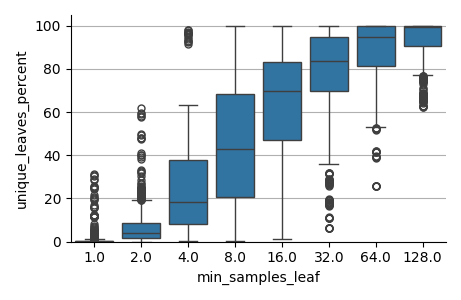
\includegraphics[width=2in]{reports/figures/leaf-uniqueness.png}
  \caption{ More unique leaf values are produced when there are restrictions on tree growth. }
  \label{fig:leaf_uniqueness}
\end{minipage}%
\begin{minipage}{.5\textwidth}
  \centering
  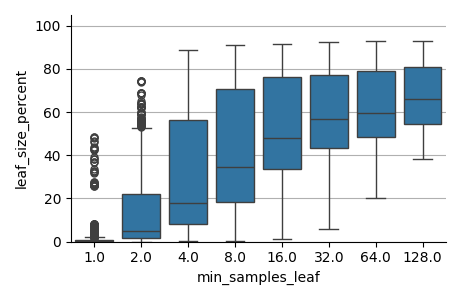
\includegraphics[width=2in]{reports/figures/leaf-proportion.png}
  \caption{The proportion of model size used by leaf nodes make up changes as restriction on tree growth. TODO: write more }
  \label{fig:leaf_proportions}
\end{minipage}
\end{figure}

TODO: results with leaf clustering (and quantization) enabled
Thesis: is pareto optimal in terms of predictive performance vs model size, when compared to majority and full soft voting
? how to show that this holds across all (or majority) of datasets

\subsection{Tests on microcontroller hardware}

REAL WORLD TEST.
? Would have to make some illustrations of this.
For example on HAR task/datasets, that on relevant microcontrollers, memory is problem before execution time. Need also to account for feature extraction time, which dominates.
Typical workflow. Set hard constraints on model size. Optimize for maximal predictive performance. Say 1kB, 10kB, 100kB - or maybe steps of 2x

VISUALIZATION. Model size vs predictive performance. And inference time vs predictive performance. Multiple model sizes. One line per framework, linked datapoints. Demonstrate Pareto optimality



%% DISCUSSION
\section{Discussion}

? claim. Model size is the typical main constraint for RF in TinyML settings.
Execution time (and power consumption) is less of a problem.

\subsection{Further work}

Here we only considered the use of Random Forest for classification.
The models are also used for regression.
Explore whether leaf clustering could also be useful for regression.


%\newpage
\section{Conclusions}


\section*{Acknowledgements}
\noindent

Martin Stensgård

% References
\newpage
\bibliographystyle{unsrt}
\bibliography{references.bib} 

\end{document}

